\begin{filecontents}{conservedvector.tex}

\centering
\begin{figure}
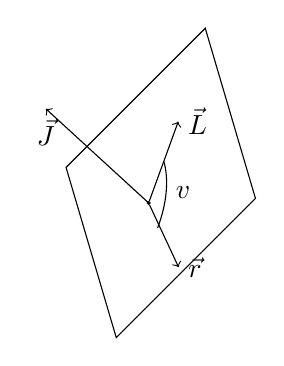
\begin{tikzpicture}[rotate around z=45, rotate around x=-45]
\draw (0,-0.3,0) -- (2.5,-0.3,0) -- (2.5,2.5,0) -- (0,2.5,0) -- cycle;
\draw[->] (1.,1.,0)node[draw,circle,inner sep=0] (o) {} -- (1.5,1.5,2)node[below] {$\vec{J}$};
\draw[->] (o) -- ++(295:0.9cm)node[right] {$\vec{r}$};
\draw[->] (o) -- ++(70:1.1cm)node[right] {$\vec{L}$}node [midway] (aux){};
\draw (aux) arc (0:-50:1) node[midway,right] {$v$};
\end{tikzpicture}

\label{fig:Lenztikz}

\end{figure}

\end{filecontents}


\begin{filecontents}{reducedproblem.tex}

%reduced problem

\begin{tikzpicture}

\node[circle,fill,inner sep=1pt,label=above:M] (M) at (0,0) {}; 
\draw (M)--++(30:1cm) node[circle,fill,inner sep=1pt,label=below:O] (O) {};
\draw[->] (O)--++(30:1.5cm) node[circle,fill,inner sep=1pt,label=above:m,yshift=1pt,xshift=1pt] (m) {} node[midway,above] {$\vec{r}$} ;

\node[circle,fill,inner sep=1pt,below=1cm of O,label=below:O] (O1) {}; 
\draw[->] (O1)--++(30:1.5cm) node[circle,fill,inner sep=1pt,label=above:m,yshift=1pt,xshift=1pt] (m1) {} node[midway,below] {$\vec{r_1}$} ;
\draw[->] (O1)--++(-150:1cm) node[circle,fill,inner sep=1pt,label=above:m,yshift=1pt,xshift=1pt] (m1) {} node[midway,below] {$\vec{r_2}$} ;
%\node (dida) at (7,0) {\parbox{8cm}{Siano m e M due masse puntiformi o a simmetria sferica: O \'e il centro di massa e $\vec{r}=\vec{r_1}-\vec{r_2}$ la distanza relativa.}};

\end{tikzpicture}

\end{filecontents}

\begin{filecontents}{ellipse.tex}

%ellisse

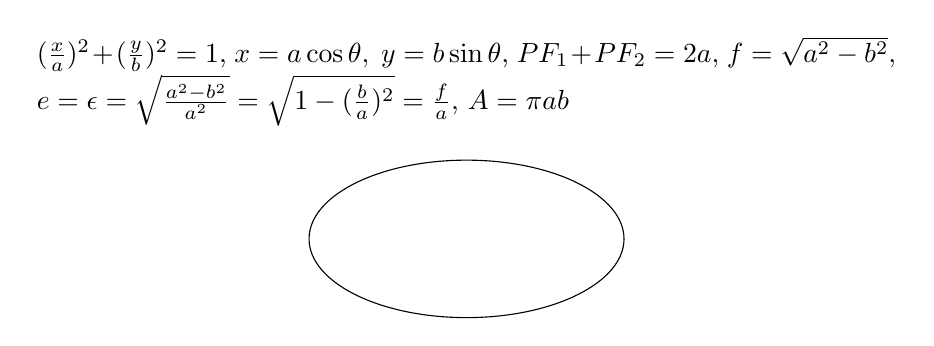
\begin{tikzpicture}

\draw ellipse (2cm and 1cm) node (o) {};
\node (prop) at (0,2) {\parbox{0.9\textwidth}{
$(\frac{x}{a})^2+(\frac{y}{b})^2=1$,
$x=a\cos{\theta},\ y=b\sin{\theta}$,
$PF_1+PF_2=2a$,
$f=\sqrt{a^2-b^2}$,
$e=\epsilon=\sqrt{\frac{a^2-b^2}{a^2}}=\sqrt{1-(\frac{b}{a})^2}=\frac{f}{a}$,
$A=\pi ab$}
};

\end{tikzpicture}

\end{filecontents}